%%%%%%%%%%%%%%%%%%%%%%%%%%%%%%%%%%%%%%%%%%%%%%%%%%%%%%%%%%%%%%%%%%%%
\section{Anode Plane Assembly (APA) Overview}
\label{sec:fdsp-apa-intro}

Anode planes (or wire planes) are the DUNE \dword{spmod} elements used to sense, through both signal induction and direct collection, the ionization electrons created when charged particles traverse the \lar volume inside the \dword{spmod}. 

The Physical Sciences Laboratory (PSL) at the University of Wisconsin and the Daresbury Laboratory in the UK have recently produced full-scale \dwords{apa} for the \dword{pdsp} project at CERN. Figure~\ref{fig:apa-photo} shows a completed \dword{apa} produced at PSL just before shipment to CERN for use in \dword{pdsp}. This effort has greatly informed the design and production planning for the DUNE \dwords{detmodule}, and \dword{pdsp} running has provided valuable validation for many fundamental aspects of the  \dword{apa} design. 

All elements of the DUNE physics program depend on a high performing system of \dwords{apa} and their associated readout electronics.  The Physics TDR (Vol. 2) describes the simulations that rigorously establish this performance.  Here we summarize some of the \dword{apa} capabilities required for the key elements of neutrino CP-violation (CPV) and associated long-baseline oscillation physics, nucleon decay, and intra-galactic supernova neutrino burst (SNB) searches.  As a multipurpose detector accessing physics from MeV to multi-GeV scales, the DUNE LArTPC cannot be optimized for a narrow range of interaction signatures in the manner of noble liquid TPCs dedicated to direct dark matter or neutrino-less double beta decay searches.  The APAs must collect ionization charge in a way that preserves the spatial and energy profiles of ionization events that range from few hundred keV point-like depositions from low energy electrons and neutrons  from SNB neutrino interactions to the double-kinked $K\rightarrow\mu\rightarrow{e}$ decay chain with its combination of highly- and minimum-ionizing particles (HIPs and MIPs) that is important for proton decay searches.  They must record enough hits on tracks within a few cm of a neutrino interaction vertex to differentiate the 1 MIP $dE/dx$ signature of a $\nu_e$-induced electron from the 2 MIP signature of a $\nu_\mu$ neutral current photon conversion to enable the $\nu_\mu-\nu_e$ separation demanded for CP-violation physics; and they must provide the pattern recognition and calorimetry for multi-GeV neutrino interaction products  spread over cubic meters of the detector needed for the precision neutrino energy estimates that allow separation of CPV effects from those related to matter effects. 
 
\begin{dunefigure}[Schematic view of a DUNE \SI{10}{kt} \dword{spmod} %single phase TPC module
]{fig:FarDet-interior}
{Left: End-on schematic view of the active argon volume showing the four drift regions and anode-cathode plane ordering of the TPC inside the detector. Right: View of the partly installed DUNE TPC inside the membrane cryostat. The \dwords{apa} are red, \dwords{cpa} are cyan, and \dword{fc} modules yellow/green.  Some of the \dword{fc} modules are folded against the cathode to provide aisle access during installation.}
%\setlength{\fboxsep}{0pt}
%\setlength{\fboxrule}{0.5pt}
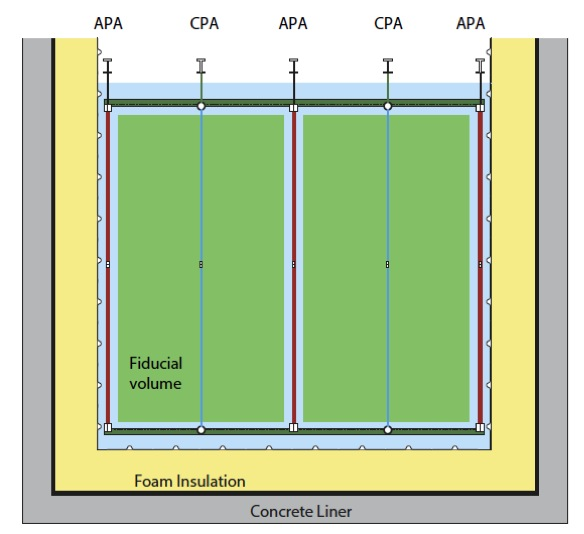
\includegraphics[width=0.445\textwidth, trim=0mm 3.7mm 0mm 0mm, clip]{sp-apa-dune-sp-end-view.jpg}\hspace{0.01\textwidth}
%\fbox{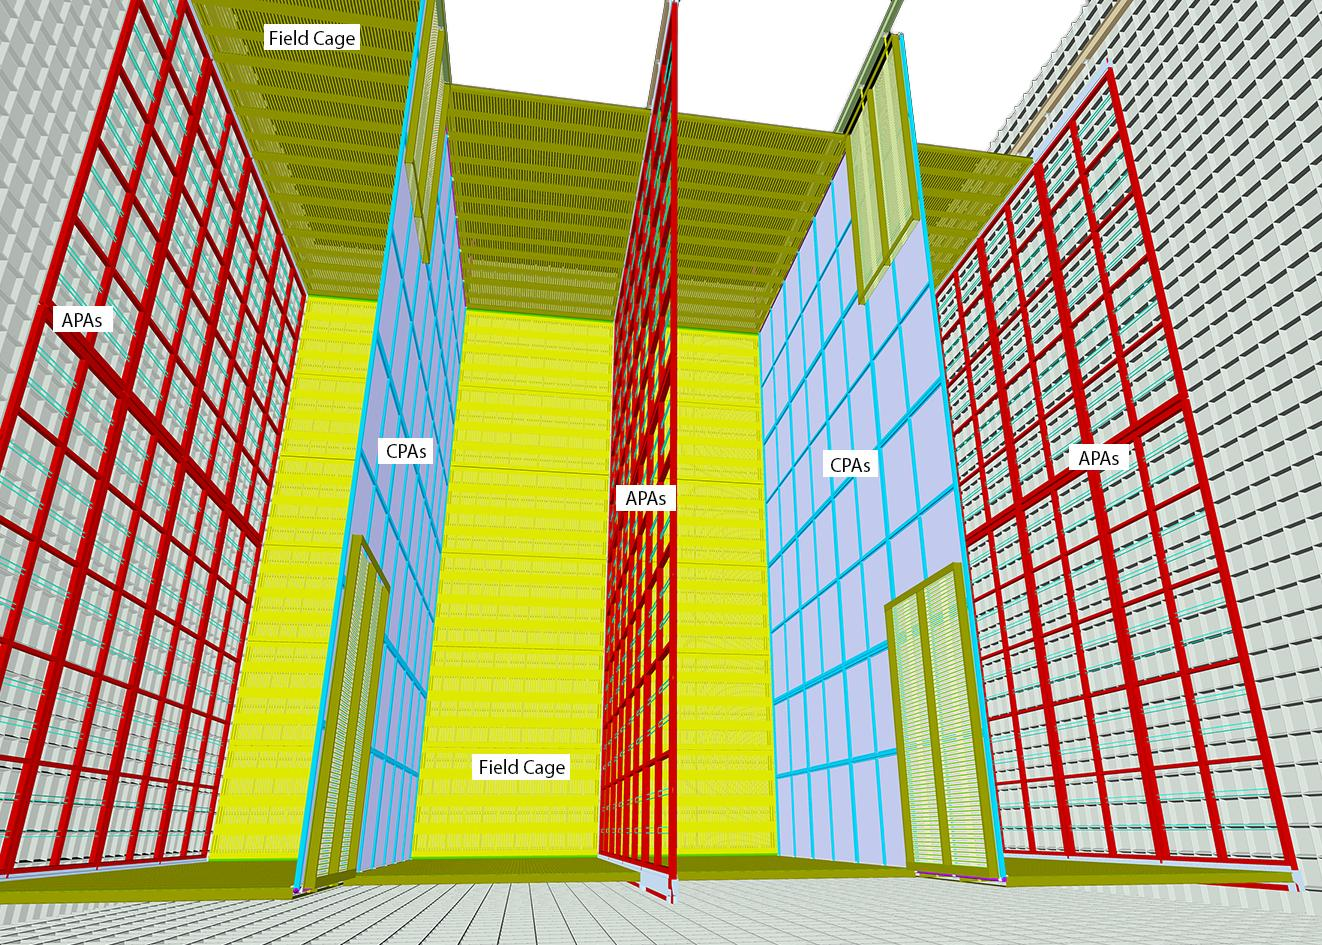
\includegraphics[width=0.52\textwidth]{sp-apa-dune-sp-floor-view.jpg}}
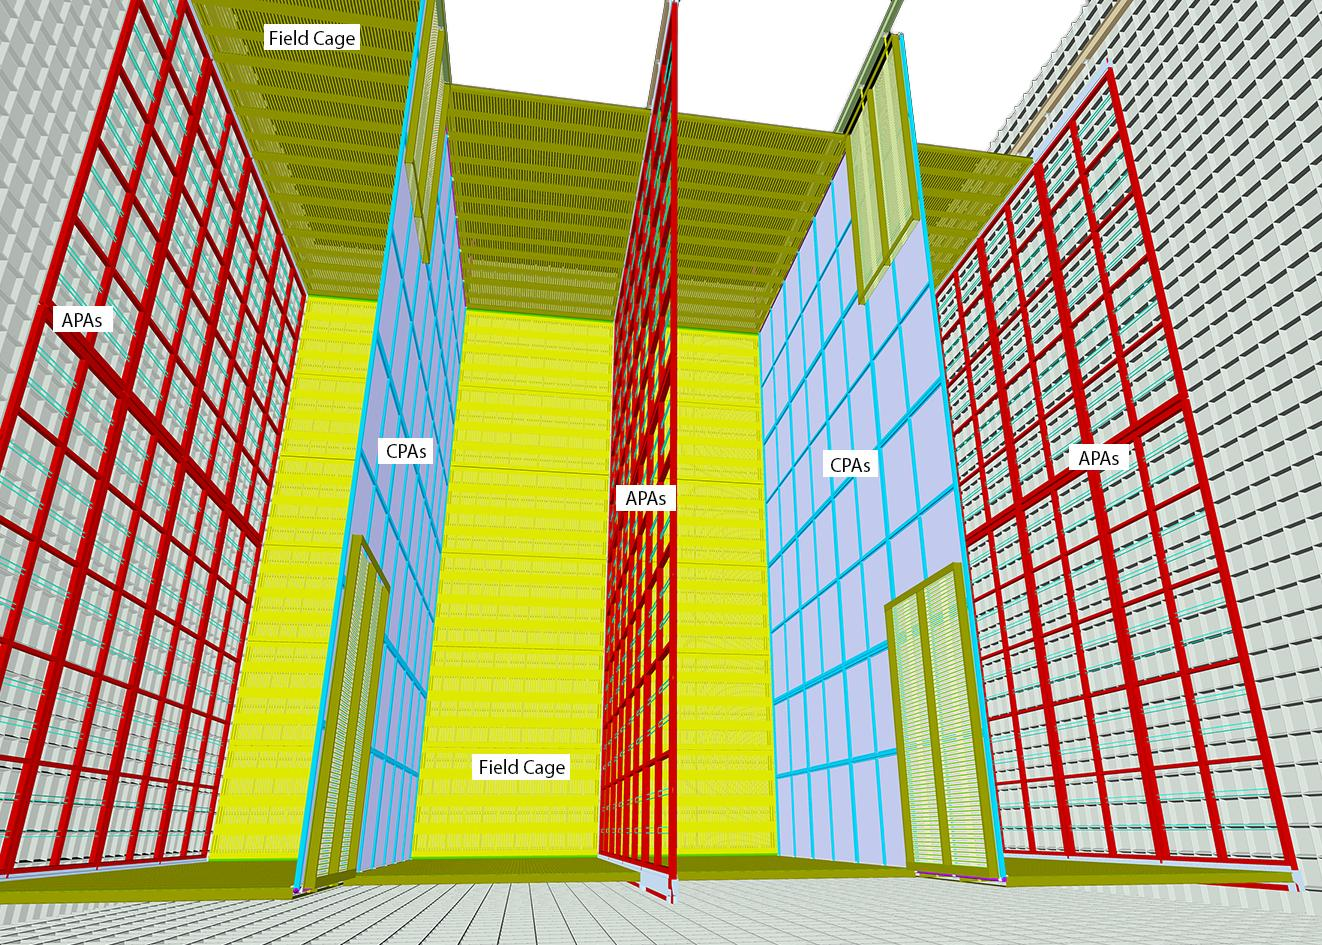
\includegraphics[width=0.52\textwidth]{sp-apa-dune-sp-floor-view.jpg}
\end{dunefigure}

Anode planes in the \dword{apa} must be well-shielded from possible high voltage breakdown events in the detector.  The \dword{apa} wire spacing and orientations must maximize pattern recognition capabilities and signal-to-noise in a cost-effective manner.  The \dword{apa} wires must maintain their positions to a level that is small compared to the wire spacing so that energy estimators based on range and multiple Coulomb scattering remain reliable over two decades of operation.  The wires must hold their tension for all this time, lest microphonic oscillations develop that degrade signal-to-noise or anode plane field distortions arise that inhibit the transmission of drifting electrons through the induction planes to the collection plane.  Any wire break would destroy fiducial volume; the \dword{apa} design must both minimize the possibility of this occurrence and contain the extent of any damage that would ensue should it happen.  An \dword{apa} implementation that meets these goals follows in the remainder of this chapter, along with a summary of significant validations achieved through dedicated simulations and ProtoDUNE construction and operations.

To facilitate fabrication and installation underground, the anode design is modular, with \dwords{apa} tiled together to form the readout system for a \SI{10}{kt} \dword{detmodule}. A single \dword{apa} is \SI{6}{m} high by \SI{2.3}{m} wide, but two of them are connected vertically, and twenty-five of these vertical stacks are linked together to define a \SI{12}{m} tall by \SI{58}{m} long mostly-active readout plane.  As described below, the planes are active on both sides, so three such wire readout arrays are interleaved with two high voltage surfaces to define four \SI{3.6}{m} wide drift regions inside each \dword{spmod}, as Figure~\ref{fig:FarDet-interior} shows in the detector schematic views. Each single-phase \SI{10}{kt} module, therefore, will contain 150 \dwords{apa}.


Each \dword{apa} frame is covered by more than \num{2500} sense wires laid in three planes  oriented at angles to each other: a vertical collection plane, $X$, and two induction planes at $\pm35.7^\circ$ to the vertical, $U$ and $V$. These enable multi-dimensional reconstruction of particle tracks.  An additional \num{960} wires that are not read out make up an outer shielding plane, $G$, to improve signal shapes on the $U$ induction channels.  The angled wires are wrapped around the frame from one side to the other, allowing all channels to be read out from one end of the \dword{apa} only (the top or bottom), thereby minimizing the dead regions between neighboring \dwords{apa}. Signals induced or collected on the wires are transferred through soldered connections to wire termination boards mounted at the end of the \dword{apa} frame that in turn connects to \dword{fe} readout electronics sitting in the \lar.  Figures~\ref{fig:tpc_apa1} and \ref{fig:tpc_apa2} illustrate the layout of the wires on an \dword{apa}, showing how they wrap around the frame and terminate on wire boards at the head end where readout electronics are mounted.

The \dwords{apa} are a critical interface point between the various detector subsystems within the \dword{spmod}.  As already mentioned, the TPC readout electronics mount directly to the \dword{apa} frames.  The \dwords{pd} for detecting scintillation light produced in the \lar are also housed inside the frames, sandwiched between the wires on the two sides, requiring careful coordination in frame design as well as requiring transparency for the \dword{apa} structures.  In addition, the electric \dfirst{fc} panels connect directly to the edges of the \dword{apa} frames.  Finally, the \dwords{apa} must support routing cables for both the TPC electronics and the photon detector systems. All these considerations are important to the design, fabrication, and installation planning of the \dwords{apa}.

\begin{dunefigure}[Illustration of the \dword{apa} wire layout]{fig:tpc_apa1}
{Illustration of the DUNE \dword{apa} wire wrapping scheme showing small portions of the wires from the three signal planes ($U,V,X$). The fourth wire plane ($G$) above these three, and parallel to $X$, is present to improve the pulse shape on the $U$ plane signals. The TPC electronics boxes, shown in blue on the right, mount directly to the frame and process signals from both the collection and induction channels. The \dword{apa} is shown turned on its side in a horizontal orientation.} 
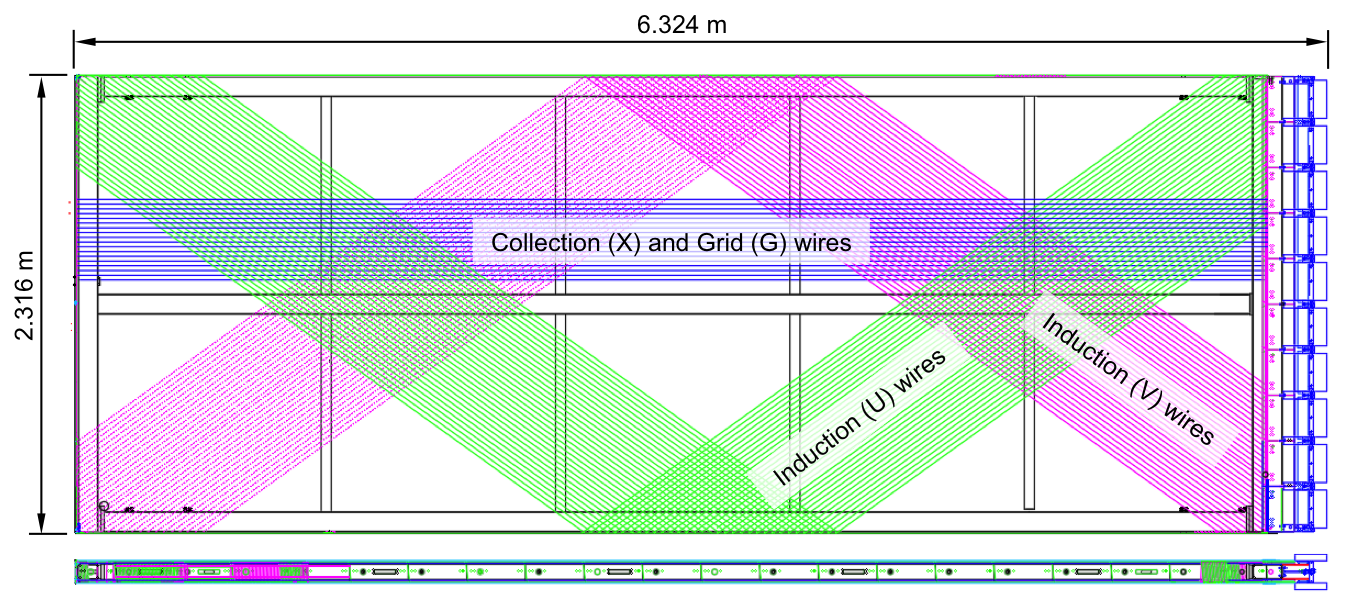
\includegraphics[width=\textwidth]{sp-apa-drawing-wire-configuration.png} 
\end{dunefigure} 

\begin{dunefigure}[Cross section view of the head end and wire layers of an \dword{apa}]{fig:tpc_apa2}
{Cross section view of an \dword{apa} frame near the head end showing the layers of wires ($X,V,U,G$ inside to out) on both sides of the frame and terminating on wire boards at the head end of the frame, which connect directly to TPC readout electronics.} 
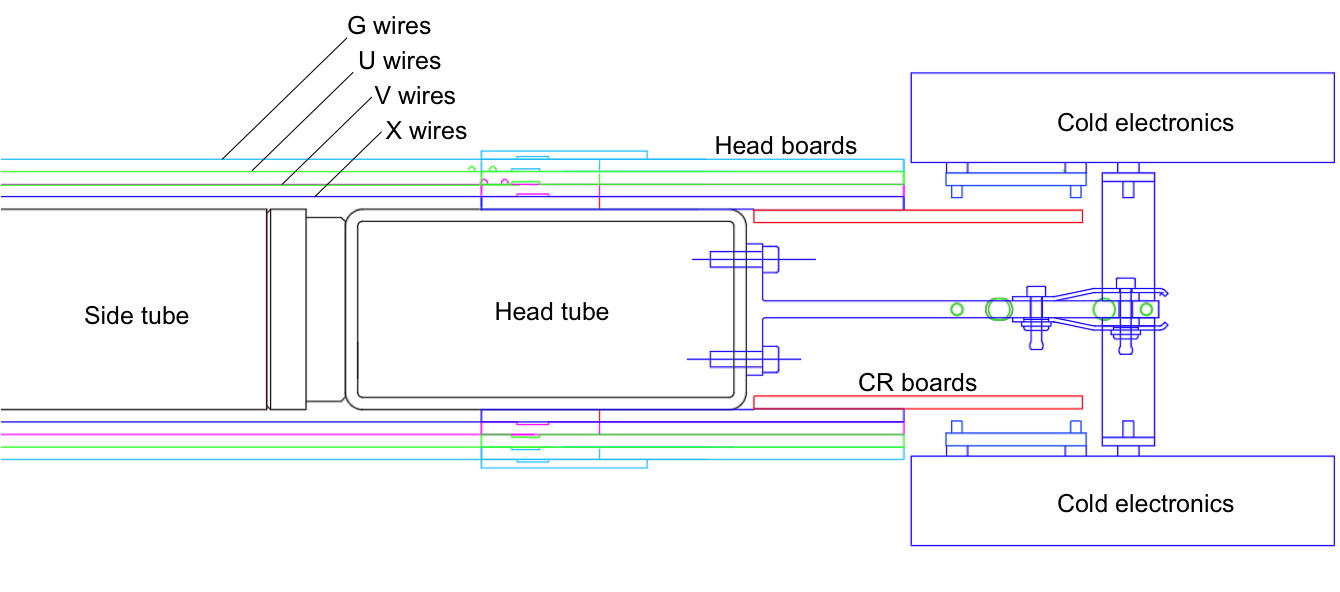
\includegraphics[width=0.95\textwidth]{sp-apa-drawing-cross-section.png} 
\end{dunefigure} 

% Anne moving higher up 12/20 per Tim: The Physical Sciences Laboratory (PSL) at the University of Wisconsin and the Daresbury Laboratory in the UK have recently produced full-scale \dwords{apa} for the \dword{pdsp} project at CERN. Figure~\ref{fig:apa-photo} shows a completed \dword{apa} produced at PSL just before shipment to CERN for use in \dword{pdsp}. This effort has greatly informed the design and production planning for the DUNE \dwords{detmodule}, and \dword{pdsp} running has provided valuable validation for many fundamental aspects of the  \dword{apa} design. 

The \dword{apa} consortium within the DUNE collaboration oversees the design, construction, testing, and installation of the \dwords{apa}. Several \dword{apa} production sites will be set up in the US and the UK with each nation producing approximately half of the \dwords{apa} needed for the %DUNE 
\dwords{spmod}.  Factory setup is anticipated to begin in 2020, with \dword{apa} fabrication for the first \SI{10}{kt} far detector module running from 2021--2023.  

This chapter is laid out as follows.  In Section~\ref{sec:fdsp-apa-design} we overview the design of the \dwords{apa} focusing on the key design parameters and their connection to the physics requirements of \dword{dune}.  In Section~\ref{sec:fdsp-apa-qa} we discuss quality assurance for the design with an emphasis on lessons learned from \dword{pdsp} construction and operations and a summary of remaining prototyping efforts being planned. Section~\ref{sec:fdsp-apa-intfc} summarizes three important interfaces to the \dword{apa}s: TPC electronics, photon detectors, and cable routing for both systems.  In Section~\ref{sec:fdsp-apa-prod} we detail the procedures for fabricating the large number of \dword{apa}s needed for the experiment including a description of the main construction sites being planned by the \dword{apa} consortium.  Section~\ref{sec:fdsp-apa-transport} describes some of the procedures for handling \dword{apa}s throughout construction and presents the design for a custom transport container. Section~\ref{sec:fdsp-apa-safety} reviews the safety considerations for \dword{apa} construction and handling, and Section~\ref{sec:fdsp-apa-org} summarizes the organization of the \dword{apa} consortium responsible for building the \dword{apa}s and provides the high-level cost, schedule, and risk summary tables. 

\begin{dunefigure}[Photo of a completed \dword{pdsp} \dword{apa}.]{fig:apa-photo}
{Completed \dword{pdsp} \dword{apa} ready for shipment to CERN.}
%\setlength{\fboxsep}{0pt}
%\setlength{\fboxrule}{0.5pt}
%\fbox{\includegraphics[width=0.9\textwidth,trim=20mm 80mm 0mm 60mm,clip]{apa-photo-complete.jpg}}
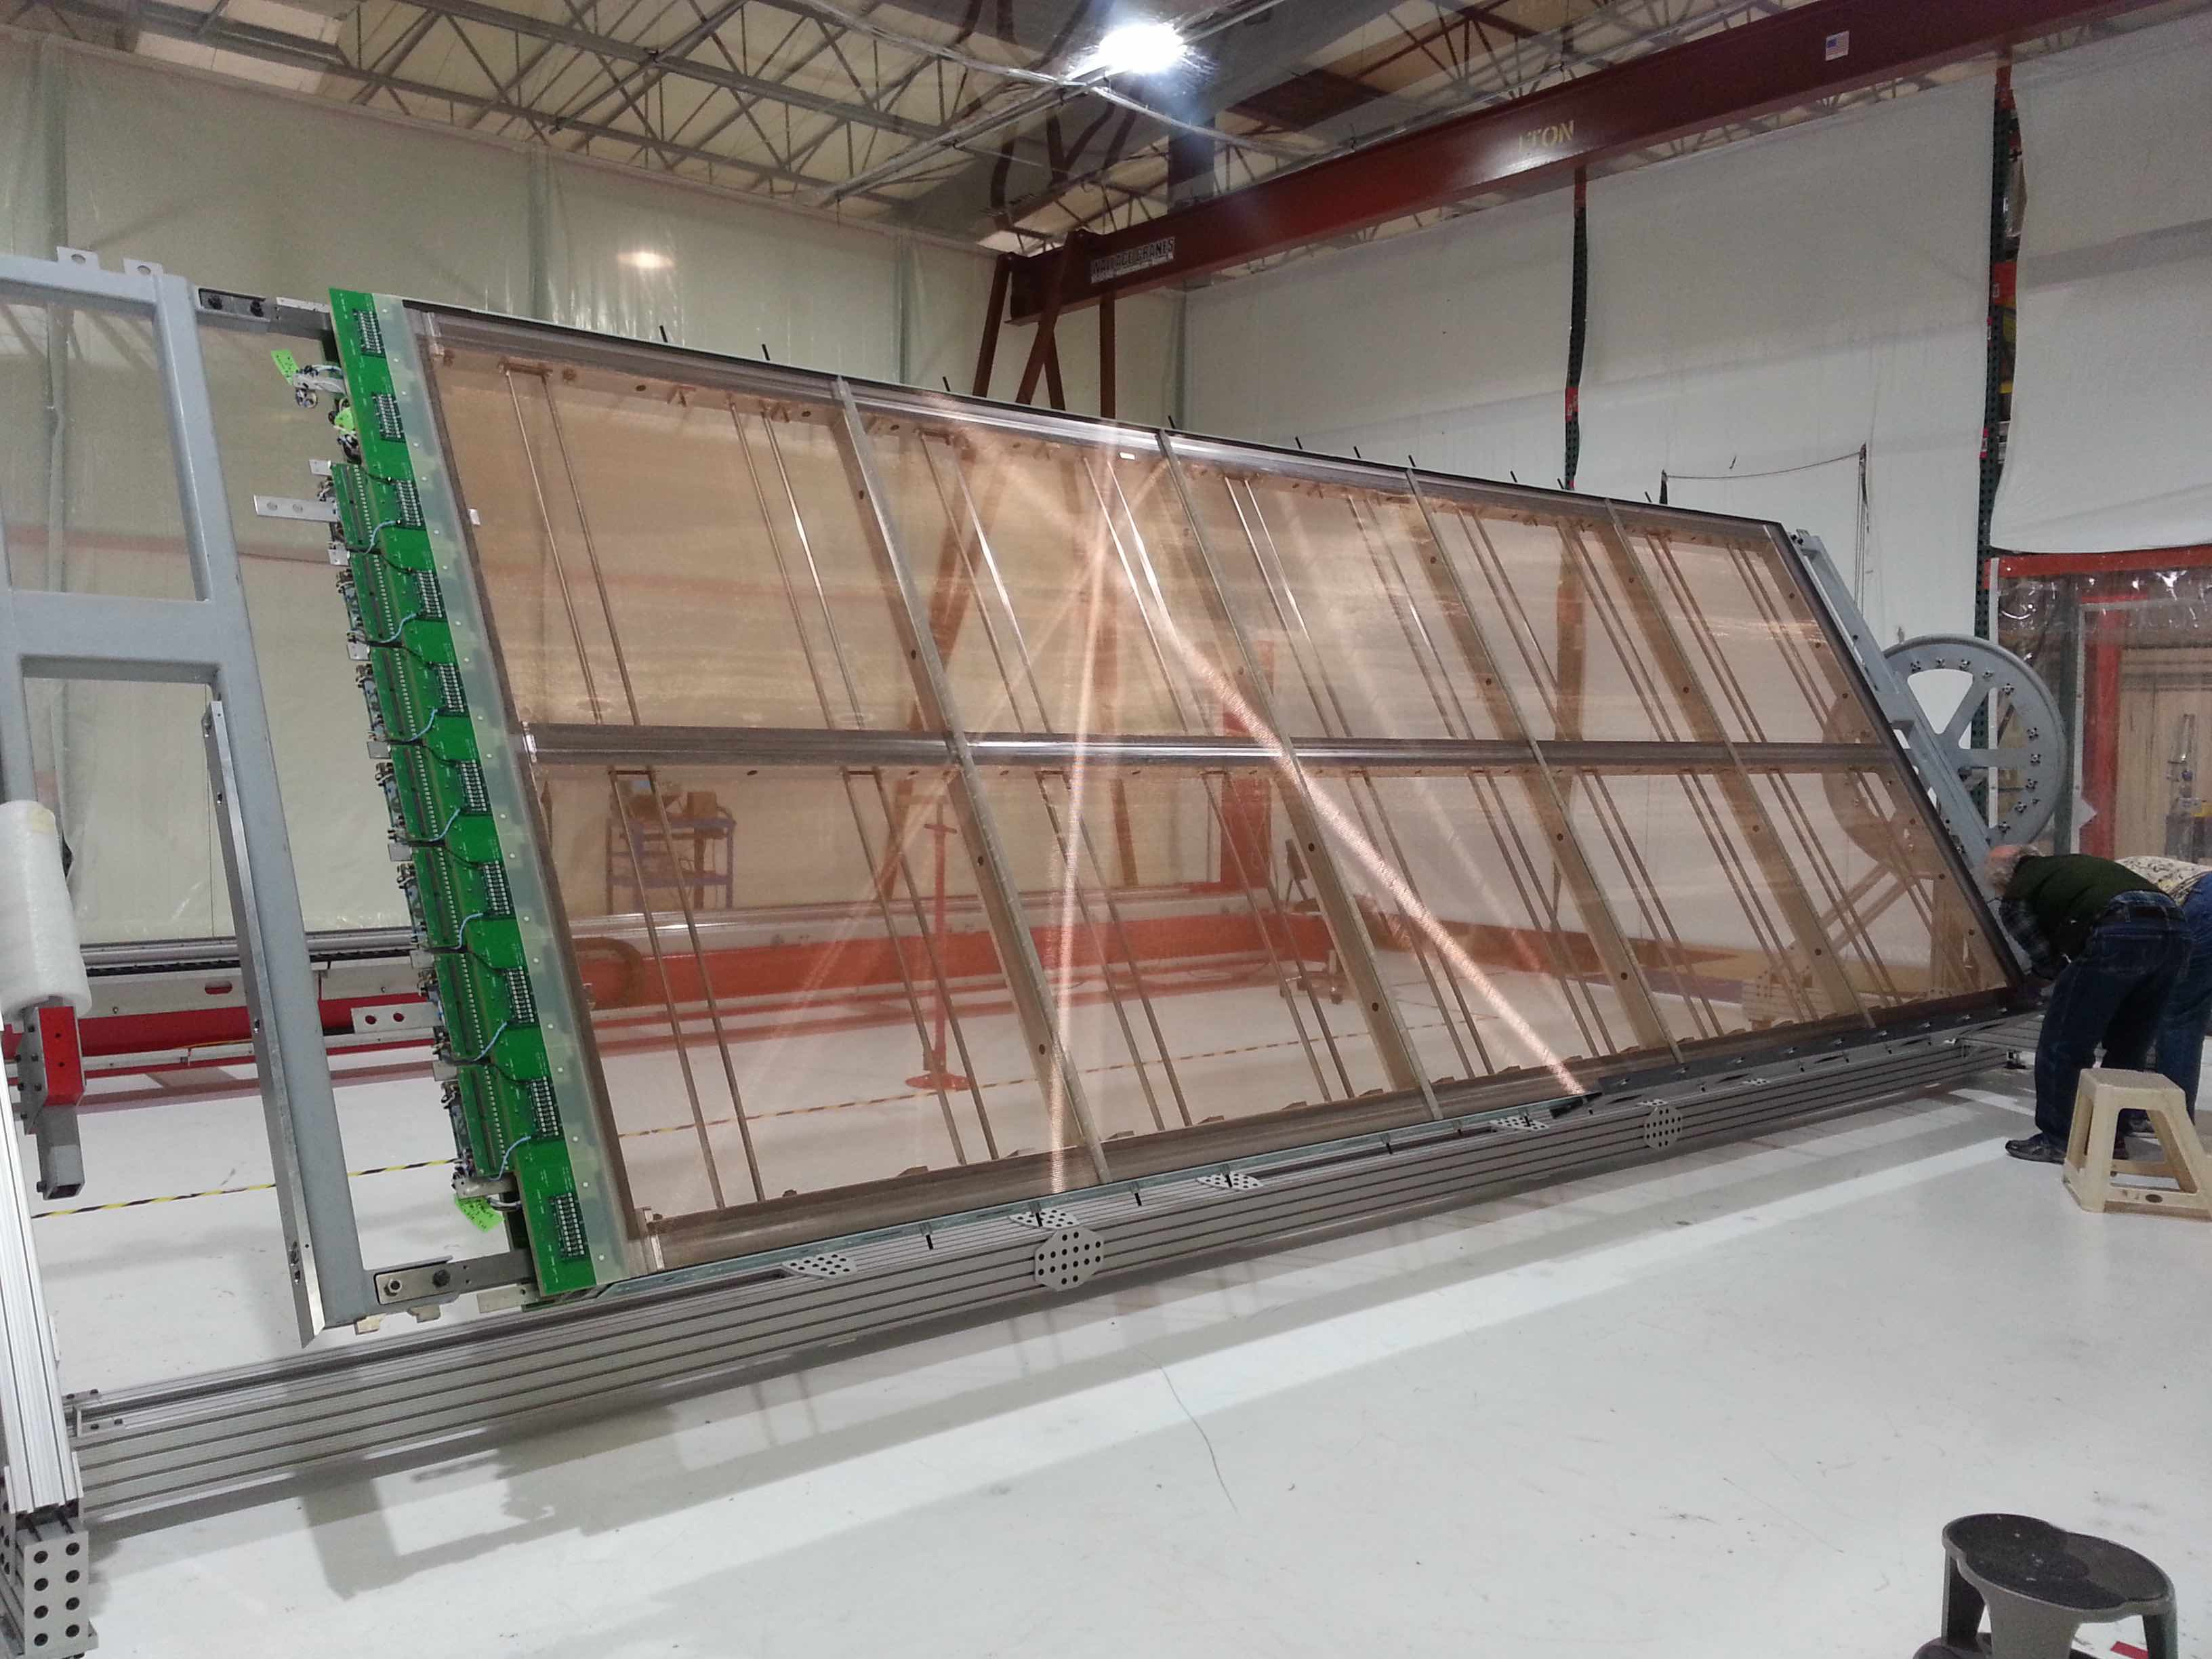
\includegraphics[width=0.95\textwidth,trim=20mm 80mm 0mm 60mm,clip]{sp-apa-photo-complete.jpg}
\end{dunefigure}
